\chapter{Business Model for the Kinect Based Exercise Game}
\section{Product}
\subsection{Value Proposition}
\section{Customer Interface}
\subsection{Customer Segments}
\subsection{Channels}
\subsection{Customer Relationships}
\section{Infrastructure Management}
This section is about how Cyberlab creates value. What resources needed and what activities that have to be preformed are described here, as well as if they will get them in-house or from a partner. 

\subsection{Key Resources}

In this section we will describe all the resources needed to make the business model work. The resources are divided into 4 different types, described in table \ref{tab:Resources}.
\newpage

\begin{table}
\centering
    \begin{tabular}{|l|l|}
        \hline
       \textbf{Type of Resource} & \textbf{Resource}  \\ \hline
       \emph{Intellectual} & Insight and experience with fall problematic in elderly \\ \cline{2-2}
        & Programming skills \\ \cline{2-2}
	 	& Creativity \\ \hline
	   \emph{Physical} & Premises \\ \cline{2-2}
	   	& Equipments, i.e. desks and computers \\ \cline{2-2}
	   	& Microsoft Xbox HW \\ \cline{2-2}
	   	& Working Environment \\ \cline{2-2}
	   	& Internet Connections \\ \hline
	   \emph{Human} & System Developers, i.e. programmers and interaction designers \\ \cline{2-2}
	   	& Administration, i.e. marketers, customer related tasks \\ \cline{2-2}
	   	& Support Person(s) \\ \hline
	   \emph{Financial} & The European Union \\
        \hline
    \end{tabular}
    \caption[Resources]{Different types of resources}
    \label{tab:Resources}
\end{table} 
\emph{Intellectual} \\ The developers needs insight and knowledge about different exercises that will strengthen muscles and improve balance in elderly. A thorough background study and research have to been conducted to acquire this knowledge. When they have enough knowledge to form the foundation of an exercise program, they can start to get creative. Creativity is needed to make the game entertaining and east to understand and conduct. In addition to that, good programming competencies is needed to develop the game. To make it as cost-efficient as possible, an experienced team should be put together. \\ \\
\emph{Physical} \\ To be able to conduct this project, the team need premises with everything that comes with it, like desks, chairs, computer, internet connection, light etc. Cyberlab is an already established business, so we can assume they already have these premises and equipments established. For this project, they will need specific hardware. The hardware consists of Xbox 360 console and Kinect sensor. In addition an environment where the game can be developed is needed. \\ \\
\emph{Human} \\ Programming skills and creativity are already described above as intellectual resources. So system developers and interaction designers are needed. An administration is needed for marketing, customer related tasks and resource management. When the game is finished it needs to be operated and maintained. These tasks can be done by one or more of the system developers. \\ \\
\emph{Finance} \\ This project is financed by the European Union. 
\subsection{Key Activities}
The game can be described as Value Chain, which means transforming inputs to a final product. From the knowledge and experience they have acquired the company wants to make a product as good and price-competitive so that their customers would choose their product instead of a product with similar value. A description of the different stages in the value chain is depicted in figure \ref{fig:ValueChainCase}. In some way it can also be thought of as kind of a Value Shop, because they are in some way solving a problem for a specific customer segment. To do this, they will work in an iterative way, where they will have to test and evaluate the game during the development process. The users have to be involved during the development. 
Activities that need to be done include research, development, testing, maintenance and updates, support, marketing and administrative tasks. 
\begin{figure}[h]
\caption[ValueChainCase]{Value chain for the Kinect based game [modified from \cite{osterwalderthesis}]}
\label{fig:ValueChainCase}
\begin{center}
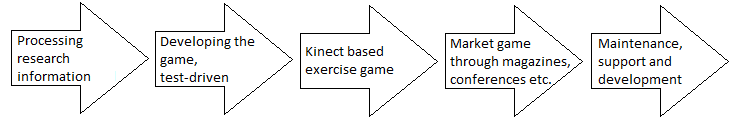
\includegraphics[scale=0.7]{valuechaincase}
\end{center}
\end{figure}
\subsection{Key Partnerships}
The main partner in this project is the partnership with the Microsoft Xbox. There are several reasons for this. First of all, they need the approvement that they are allowed to develop games for their video game console, and second, they need Microsoft Xbox’ hardware and development environment. They will also have to form an agreement with Microsoft Xbox on how they can sell the product. \\ \\ As mentioned in the introduction, this project is a collaboration between many different entities, where Norut, a national research group, is one of them. Their job in this project is to provide Cyberlab with …... finne ut av dette........ \\ \\ Physiotherapists are their customer segment, but they can also serve as a partner. Becoming partners with different clinics, will make the the marketing and selling easier, because then the actual customer believes in it. \\ \\ If professionals, physiotherapists believes in this, then the government should believe in it. Getting this game into a medical program financed by the government will make this game very credible for the end user. The Government could then provide the game to hospitals, care centers, physiotherapy clinics, training groups, and for special cases, when the elderly for example stays in their own house. \\ \\ Becoming partners with the Norwegian Government will first require that the physiotherapists believes in it, so they will first have to join the team. But it is not a requirement that physiotherapists become a partner. But some kind of collaboration has to be established with the physiotherapists. This will typically happen in the research, - development -and testing phase. \\ \\ Having the Norwegian Government as a partner will solve some of the financial issues. Most hospitals, physiotherapy clinics and training groups are managed and financed by the Government. With them believing in the game and including it as a helping tool that will prolong and improve elder's life it will be easier to hit the target users. 
\section{Financial Aspects}
In this section all the outgoing and incoming money will be described. All the previous blocks described are contributing to a cost or an income. We will try to provide an as realistic and detailed estimate of both costs and income.
\subsection{Revenue Streams}
\subsection{Cost Structure}
Cost structure takes all elements that generates cost specific to this game into account. Cyberlab is an already established business and we can therefore assume that there are not any additional costs associated with premises and some of the “regular” equipments. First we distinguish between fixed and variable costs. In this case fixed costs are associated with salaries to the project team, which includes project manager, developers, researchers, interaction designers and marketers. We define these as fixed costs because the employers are hired to do this job over a fixed period of time. Other fixed costs include hardware and software that are needed to set up an environment for developing of the game. (Prøve å få faktiske tall fra tor ivar her..) Variable costs in this case includes Xbox hardware depending on the demand from the customers. 

